\documentclass[11pt]{article}
\usepackage{colacl}
\usepackage{graphicx}
\usepackage[utf8]{inputenc}
\usepackage[dvipsnames]{xcolor}
\usepackage[inline]{enumitem}
\sloppy

%used for identifying drafting or notes
\newcommand{\drafting}[1]{\textcolor{OliveGreen}{#1}}

\title{COMP30027 Assignment 2 Report}
\author
{Anonymous}

\renewcommand\labelenumi{(\theenumi)}

\begin{document}
\maketitle

\section{Introduction}
The goal of this project was to predict the star ratings of a review of a restaurant based on the review text. The data available for learning and evaluation consisted of approximately 250000 Yelp reviews, and is made available by \cite{medhat_sentiment_2014} and \cite{rayana_collective_2015}. Each review consists of the review text, a rating (1, 3 or 5 stars) and review metadata (which was not used). We sought to investigate to what extent it was possible to predict the rating of a review from the review text alone. 

\section{Background}
This task is a type of sentiment analysis: the task of predicting sentiment from text. Performing sentiment analysis first requires extracting features from text. One common method is to convert text to a Bag-of-words (BOW), in which entries consist of word frequencies. This is method is simple, although has the disadvantage of producing high dimensional features and not representing word ordering \cite{le_distributed_2014}. A more sophisticated technique is Paragraph Vector Encoding (PVE), which uses a neural network to embed texts within an vector space in such a way that semantically similar texts are closer \cite{le_distributed_2014}.

Sentiment analysis tasks tend to deal with high dimensional, sparse, and correlated features. This often leads to classes being linearly separable, making support vector machine (SVM) models a popular choice \cite{medhat_sentiment_2014}. In terms of probabilistic classifiers, logistic regression models tend to perform well (compared to other probabilistic classifiers like na\"{i}ve Bayes) on sentiment analysis tasks since they do not assume features are independent \cite{medhat_sentiment_2014}.

\section{Method} \label{sec:method}
We investigated models based on logistic regression (Section \ref{subsec:method-lr}) and SVM (Section \ref{subsec:method-svm}) techniques, in each case using the implementations made available through the Scikit-Learn Python library \cite{sklearn_pedregosa_scikit-learn_2011}. These models used PVEs of the review text, which was produced using the implementation made available through the Gensim Python library \cite{gensim_rehurek_software_2010}. 

\subsection{Feature Selection} \label{subsec:method-features}

To decide between BOW and PVE representations of review text, we used Principle Component Analysis and Singular Value Decomposition to visualise the features and observed that PVE resulted in more distinct class clusters. Empirically we found including BOW features decreased performance in simple models, so PVE was used exclusively in all subsequent models. This means that the dimension of the PVE-space is a hyperparameter for all of our models. This can be interpreted as a measure of complexity of the model, since as the dimension increases the PVE is better able to represent the semantic nuance of the text.


\subsection{Logistic regression} \label{subsec:method-lr}
We investigated a Multinomial Logistic Regression (MLR) model. MLR has one hyperparameter $C$, which determines how strongly the model fits to the training data and avoids misclassifying training instances.

Several techniques exist for multi-class classification using Logistic Regression, such as training multiple binary Logistic Regressors (one for each class label) using a one-versus-rest scheme and predicting based on the model with the highest score, or Ordinal Logistic Regression, which is particularly suited for ordinal class labels.
One-versus-rest models are less efficient, tending to have larger standard errors \cite{zbMATH01817585}, and so were not investigated further.
Ordinal Logistic Regression is not implemented as part of the Scikit-Learn Python library and thus was not investigated due to time constraints.

\subsection{Support vector machine} \label{subsec:method-svm}
We investigated three variants of SVM classifier: a SVM with a linear kernel and one-verses-rest multi-class classification (Linear-SVM), a SVM model with a radial basis function (RBF) kernel and one-verses-rest multi-class classification (RBF-SVM), and a SVM with a linear kernel separating the positive and negative sentiment classes, in which marginal instances are classified as having neutral sentiment (Binary-SVM). 

All three SVM-based model have a regularisation coefficient $C$ as a hyperparameter, which determines the trade-off between margin maximisation and training error minimisation. The RBF-SVM also has the kernel hyperparameter $\gamma$\footnote{In the Scikit-Learn implementation $\gamma/(\textrm{var}(X) \cdot \texttt{num\_features} )$, which was used as the value for the \texttt{gamma} parameter in the model constructor.}. The Binary-SVM has the probability threshold hyperparameter $p_T$, which is the probability a negative or positive class prediction must exceed to be classified as that class.

\subsubsection*{Justifying SVM model selection}
In contrast to BOW, PVE is well suited to classification by an SVM model since paragraph vectors have meaningful geometric relationships to eachother \cite{le_distributed_2014}, and SVM models attempt to exploit the geometry of the feature space by fitting a separating hyperplane. PVE is also designed to transfer relationships in the meaning of text to linear relationships between paragraph vectors \cite{le_distributed_2014}. If we suppose that negative and positive sentiment reviews have exactly opposite meanings then we would expect the review text of these classes to be linearly separable with PVE. Preliminary testing of different kernel functions indeed showed that an SVM classifier with a linear kernel performed the best in every metric, however an SVM classifier with a RBF kernel came close to linear in performance.

Under these assumptions, it seems plausible that the neutral sentiment reviews will lie close to the hyperplane which separates the positive and negative sentiment reviews. This encourages the consideration of model that uses linear SVM to distinguish positive and negative reviews, and classifies marginal instances as neutral. We opted to use a probabilistic variant of SVM which estimates the probability of an instance belonging to each class based on its distance to the hyperplane \cite{platt_probabilistic_1999}. This allowed us to use a probability threshold for neutral classification as a hyperparameter, rather than a distance threshold, which means the value of this threshold is independent of the specific text embedding\footnote{The specific embedding of a particular text is only relevant in the context of the training corpus used to compute the embedding function \cite{le_distributed_2014}.}. Despite its appeal, results in the literature suggest that a classifier like this will always perform worse than one using a standard multi-class approach \cite{koppel_importance_2006}.

\subsection{Stacking model}
We investigated stacking as an ensemble technique to improve the performance of our base classifiers. We stacked all combinations of our best classifiers, Logistic Regression, RBF SVM and Linear SVM and used an MLR for the meta-classifier. For every combination, we used the best respective hyperparameters for each base classifier, including the PVE dimension.

\section{Results}
In order to identify the optimal feature space dimension for each model, we first evaluated our model (with hyperparameters untuned) on PVEs of dimensions 25 to 300 in steps of 25 encodings using an 80:20 stratified random holdout\footnote{\label{fn:training-d2v}Only using the training set to compute the PVE mapping}. A random holdout method, rather than cross-validation, was used due to the computation expense of computing PVEs: producing cross-validation splits for many dimensions was out of the question. Using stratified splits was particularly important due to difference in proportion of the three classes (69\%, 29\% and 8\% positive, negative and neutral respectively). For the RBF-SVM and Binary-SVM models this dimension was 125, and for the Linear-SVM and MLR models this dimension was 150.

We then computed the PVE for a 5-fold stratified cross validation split at that dimension\textsuperscript{\ref{fn:training-d2v}}. This pre-computed split was then used to tune the remaining hyperparameters. The use of cross-validation helps avoid overfitting the training data when doing this. We found that the best hyperparameter values were: for Linear-SVM $C = 0.009$, for RBF-SVM $(C, \gamma) = (1.25, 0.6)$ (Figure \ref{fig:rbf-gridsearch}), for Binary-SVM $(C, p_T) = 0.0025, 0.9)$ (Figure \ref{fig:binary-gridsearch}), and for MLR $C = 0.015$.
\begin{figure}
	\centering
	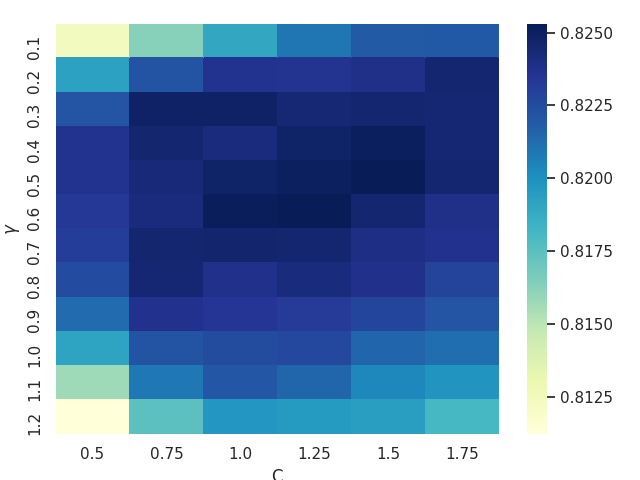
\includegraphics[width = 0.3\textwidth]{fig-rbf-gridsearch.png}
	\caption{RBF-SVM Gridsearch}
	\label{fig:rbf-gridsearch}
\end{figure}

\begin{figure}
	\centering
	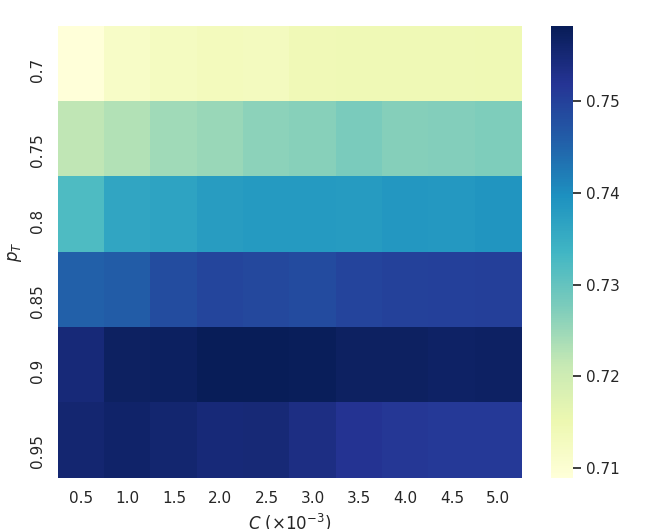
\includegraphics[width = 0.3\textwidth]{fig-binary-gridsearch.png}
	\caption{Binary-SVM Gridsearch}
	\label{fig:binary-gridsearch}
\end{figure}

After tuning the hyperparameters, we evaluated the final model trained on PVEs of dimensions from 25 to 300 in steps of 25 to produce the learning curve in Figure \ref{fig:learning-curve}. 
\begin{figure}
	\centering
	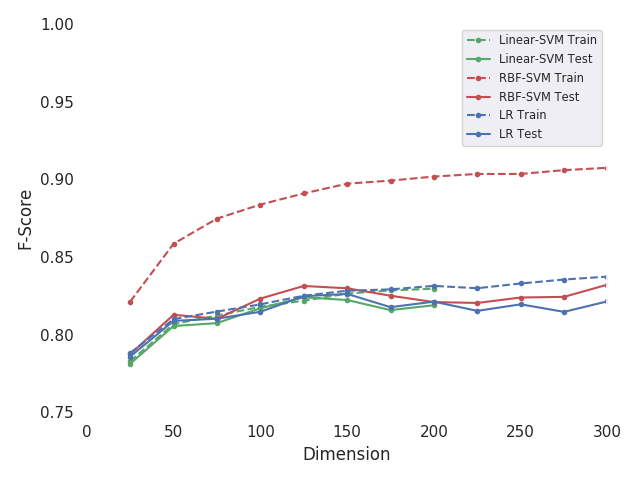
\includegraphics[width = 0.3\textwidth]{learning-curves.png}
	\caption{Learning curve}
	\label{fig:learning-curve}
\end{figure}

We also evaluated our model on the 5-fold cross validation split at the optimal dimension, the results of which can be seen in Figures \ref{fig:binary-cm}, \ref{fig:linear-cm}, \ref{fig:rbf-cm}, \ref{fig:lr-cm}. 
\begin{figure}
	\centering
	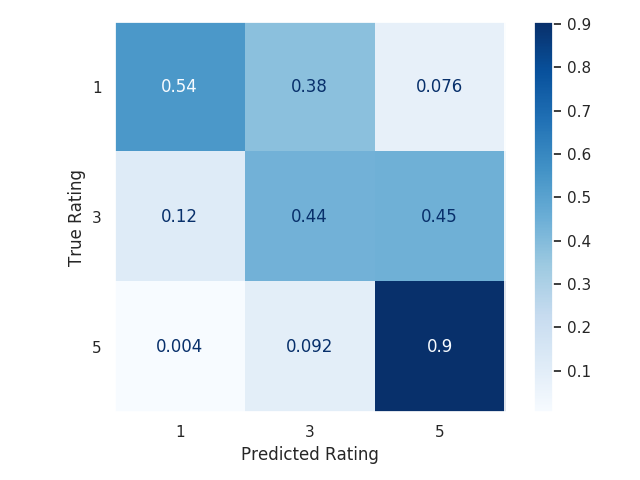
\includegraphics[width = 0.3\textwidth]{fig-binary-cm.png}
	\caption{Binary-SVM Confusion Matrix}
	\label{fig:binary-cm}
\end{figure}

\begin{figure}
	\centering
	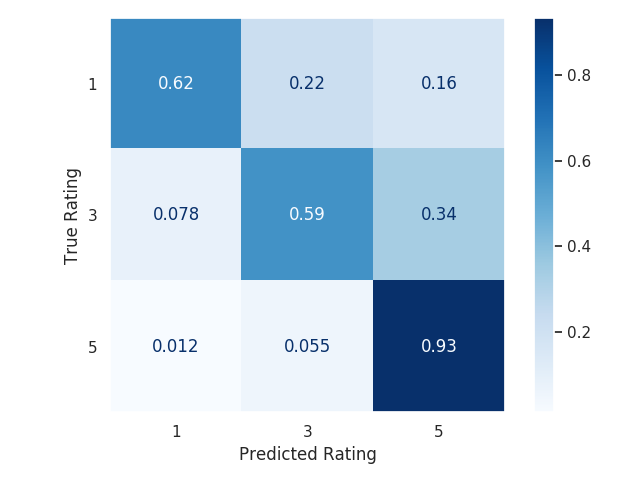
\includegraphics[width = 0.3\textwidth]{fig-linear-cm.png}
	\caption{Linear-SVM Confusion Matrix}
	\label{fig:linear-cm}
\end{figure}

\begin{figure}
	\centering
	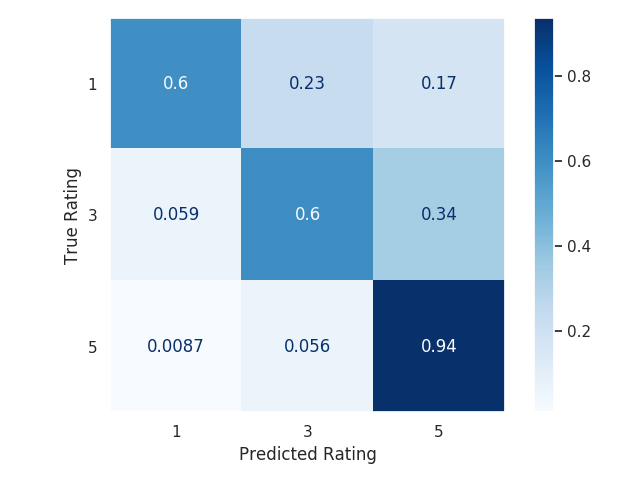
\includegraphics[width = 0.3\textwidth]{fig-rbf-cm.png}
	\caption{RBF-SVM Confusion Matrix}
	\label{fig:rbf-cm}
\end{figure}

\begin{figure}
	\centering
	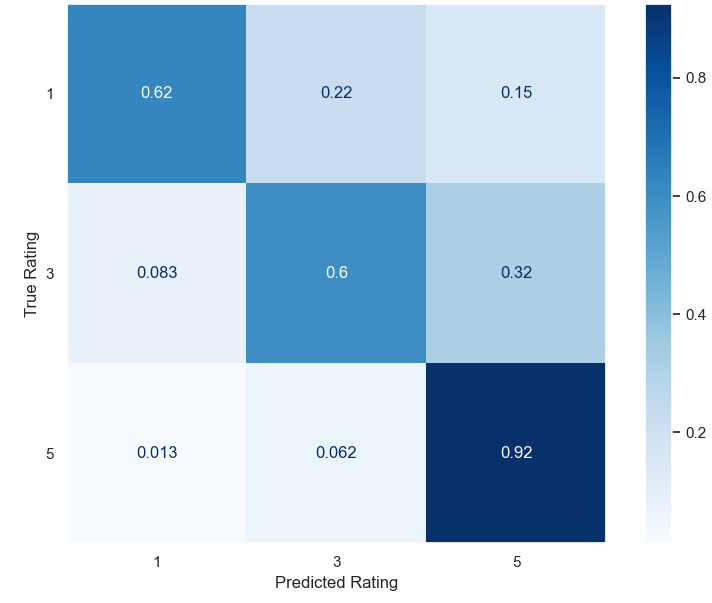
\includegraphics[width = 0.25\textwidth]{fig-lr-cm.png}
	\caption{Logistic Regression Confusion Matrix}
	\label{fig:lr-cm}
\end{figure}


We evaluated each stacked model using cross validation. Stacking models took a long time to train which made investigating different hyperparameters for base models difficult. When the base classifiers had different optimal dimensions for PVE, we selected the dimension optimal to the classifier with better sole performance. Stacked RBF-SVM and Linear-SVM had a higher accuracy and F1-score than all other stacked models, including all 3 models stacked together. The results for this model can be seen in Figure \ref{fig:stack-cm}.
\begin{figure}
	\centering
	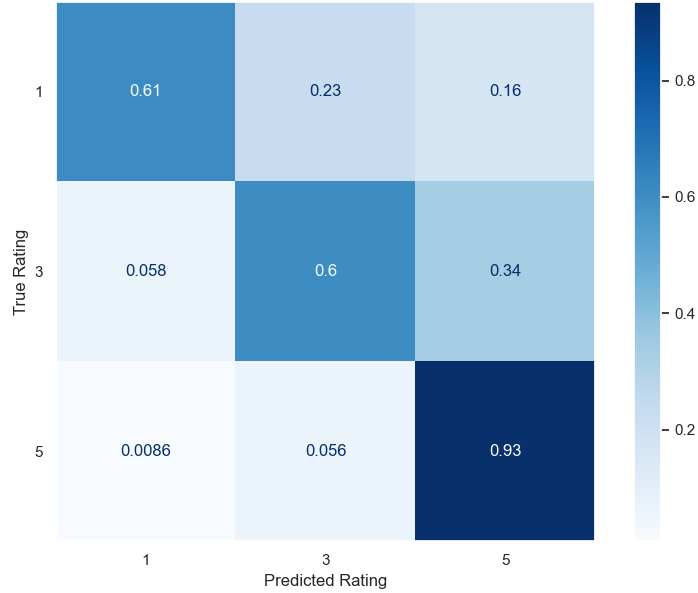
\includegraphics[width = 0.22\textwidth]{fig-stack-cm.png}
	\caption{Stacking Confusion Matrix}
	\label{fig:stack-cm}
\end{figure}

\section{Analysis}
All models achieved better accuracy than the Zero-R baseline model, which has an accuracy of $69 \%$, which shows that the models were to some degree using features to effectively make predictions. All models, including the stacking models, did not exceed an F-Score of 0.83 on held-out data. Since stacking does not improve model performance significantly, and model performance is very similar, this suggests that all models are drawing roughly the same decision boundary between the classes. This means the stacking model cannot exploit the strengths and minimise the weaknesses of the differences in the models, leading to approximately the same performance as its component models. Another possible reason for this is that the similar performance reflects the inherent difficultly of the classification task (with the selected features). It is likely that it is not possible to predict the rating entirely from the review text. Even for a human reader, the rating provides context by which to judge the sentiment of the review. For example the same review text may be interpreted as a genuine complement alongside a 5 star rating, but as sarcastic alongside a 1 star rating.

Despite having the best performance of the SVM-based classifiers on unseen data, it appears that the RBF-SVM tends to overfit the training data. In Figure \ref{fig:learning-curve} we can see that the performance of RBF-SVM on the training set is significantly higher than on the test data. This is in contrast to the other classifiers, which have very similar performance on the training and testing data. This suggests RBF-SVM is learning a decision boundary which is tailored to the training data, and so, despite performing marginally worse, Linear-SVM has better generalised from the training data. This is consistent with the assumption that the data should be linearly separable discussed in Section \ref{subsec:method-svm}.

As we can see in Figures \ref{fig:binary-cm}, \ref{fig:linear-cm}, \ref{fig:rbf-cm}, \ref{fig:lr-cm} and \ref{fig:stack-cm} the main difference in performance between the models comes from their ability to distinguish the negative and neutral sentiment classes. All models were, to varying degrees, biased towards predicting the text to be more positive than it was, with the upper triangle of the confusion matrix containing the most incorrect predictions. One reason for this is that the data contains mostly positive and neutral examples. If the prior probability of a class is higher, it makes sense that a classifier would predict it more frequently and thus be more often incorrect when predicting this class. Another factor may be that the distinction between adjacent classes is fuzzy. These two factors combined would lead to the observed tendency of models to frequently predict one class more positive than the true class.

The Binary-SVM model (F-score of 0.758) performed worse than the Linear-SVM model (F-score of 0.821) which is consistent with results in the literature \cite{koppel_importance_2006}. This means that the assumptions about the text data discussed in Section \ref{subsec:method-svm} which would lead to good performance of the Binary-SVM model are too strong. It is likely that the language used in positive and negative reviews is not completely opposite, so PVEs of these reviews do not lie along a line. Even if this were the case, there is no reason an SVM model using a standard multi-class classification technique could not learn the same decision boundary as a model like Binary-SVM.

One major improvement we could make would be to attempt to simplify texts linguistically prior to producing the PVEs. In the simplest case this could involve using an automated spell checker on the reviews, and in more complex cases undoing negatives (``not bad'' $\rightarrow$ ``good''), and identifying common phrases or idioms. Given enough examples, the paragraph vector encoding should be able to account for this without preprocessing, since words and phrases with similar meanings should be close in the feature space. However it is likely that there are not enough examples of misspellings and unusual phrasings in the training set to do this effectively in all cases.

\section{Conclusion}
We found that all investigated models were able to predict the rating from the review text along better than a Zero-R baseline classifier. Except for Binary-SVM, all models had very similar performance. This invites the question of whether it is possible to do better than the models discussed here with the selected features, or if that limit is due to the intrinsic predictability of the data with the features used. 

This work also raises the question of to what extent linguistic preprocessing can improve performance on this dataset.

%put any citations here which must be included in the bibliography but won't necessarily be referenced

%citations for the dataset
\nocite{mukherjee_what_2013}
\nocite{rayana_collective_2015}

%citations for software libraries
\nocite{sklearn_pedregosa_scikit-learn_2011}
\nocite{gensim_rehurek_software_2010}
\bibliographystyle{acl}
\bibliography{report}

\end{document}
